\documentclass[11pt,oneside, final]{fithesis2}  
\usepackage[english]{babel} % package for multilingual support  
\usepackage[utf8]{inputenc} % Windows OS encoding  
\usepackage[T1]{fontenc}  
\usepackage{lmodern}
\usepackage{cmap}

\usepackage[plainpages=false,pdfpagelabels,unicode]{hyperref}
\usepackage[numbers, sort]{natbib}
\usepackage{graphicx}
\usepackage{multirow}
\usepackage{siunitx}

%\usepackage[linenumbers,noindent]{stdpage} %1800 character standard pages

%\renewcommand{\baselinestretch}{1.2}	% 1.2 radkovani
 
\thesistitle{Engine for drawing isometric game graphics in SVG} % enter thesis title  
\thesissubtitle{Master's thesis}  
\thesisstudent{Bc. Vít Svoboda}    % name of the author  
\thesiswoman{false}          % defines author?s gender  
\thesisfaculty{fi}  
\thesisyear{spring 2015}  
\thesisadvisor{Mgr. Marek Grác, Ph.D.} % fill in advisor?s name  
\thesislang{en}                 % thesis is in English  
 
\begin{document}  
\FrontMatter  
\ThesisTitlePage  
 
\begin{ThesisDeclaration}  
\DeclarationText  
\AdvisorName  
\end{ThesisDeclaration}  
 
\begin{ThesisThanks}  
I would like to thank my advisor for patience and academic guidance. I would also like to thank Ing. Ondřej Žižka for technical consultations.
\end{ThesisThanks}  
 
\begin{ThesisAbstract}  

\end{ThesisAbstract}  
 
\begin{ThesisKeyWords}  
5-10 key words, one key word can be multiple words. Key words are comma separated. Not the list of used technologies!
\end{ThesisKeyWords}  
 
\MainMatter
 
\tableofcontents          % prints table of contents  
 
\chapter{Introduction}
Specification of HTML5 introduced two new elements to display graphics natively in the browser: \texttt{canvas} and \texttt{svg}\cite{w3_html5}. Before that the browser games had to be built using third party solutions to display the game graphics\cite{pagella}. With the broad adoption of the new standard, the game development focus shifted to the \texttt{canvas} element\cite{pagella}. The question this thesis attempts to answer is whether it is possible to utilize the latter of the new elements in the same way as the first one has successfully been so far. Chapter \ref{theory} briefly describes the current state of graphics engine usage and expectations. Furthermore the chapter focuses on a graphics style named after the projection method used -- the isometric graphics and outlines its origin and usage in the course of video game history. This method can be applied in the web environment to achieve balance between visual appeal and rendering speed. At the end the chapter elaborates on the specifics of web graphics and the way they are usually presented to the users' clients.

Chapter \ref{solution} describes a graphics engine that would allow rendering isometric game graphics to the \texttt{svg} element and could prove such usage is possible. This method of rendering graphics could serve as an alternative to the commonly used \texttt{canvas} as well as making certain aspects of the game development substantially easier. Chapter \ref{tech} summarizes technologies considered to be used within the engine implementation. The actual implementation and its consequences for the engine user -- a game developer -- are described in Chapter \ref{implementation}. The proposed engine implementation is subjected to testing and stress to assess the usability by real applications in Chapter \ref{testing}.

\chapter{State of the art}
\label{theory}

Modern video games are designed to be data driven\footnote{Data-driven program determines execution flow based on provided data. The data describe program behavior. Therefore an unchanged code can perform different tasks when given appropriate data.\cite{charniak}}. That way as much code as possible can be used again in similar games. The common functionality can be packed in a software component called game engine\cite{gregory} and distributed separately from the game itself for other developers. A game engine is responsible for collision detection, physics calculation, game logic script execution and, for the focus of this work most importantly, rendering. Part of a game engine that encapsulates the last mentioned responsibility is called graphics or rendering engine.

\section{Graphics engine}
Graphics engine is a software component responsible for transformation of a logical model of a scene to an image on the screen. Graphics engines used in native applications heavily depend on middleware like OpenGL or DirectX\cite{gregory}.

\subsection{Typical functionality}
\label{enginefunctionality}
The input for a graphics engine is a set of objects on the scene, data representing their appearance\footnote{Sprites, meshes and textures} and a camera position. The engine has to determine what objects or their parts are currently visible from the point of view of the given camera. A properly placed visual representation needs to be created for these objects. The output is a bitmap stored in memory containing graphic representation of all related objects. It can be prepared directly or more usually, rather than manipulating the bitmap directly, done via a series of calls to some underlying API\footnote{Application Programming Interface}. Optionally the engine can perform various post-processing on the output, such as anti-aliasing, shading etc.\cite{gregory} More complex post-processing is usually performed only in 3D applications. When rendering a real-time image, the process has to be repeated several times per second to maintain perception of a fluid animation. Simply put, the higher frame rate\footnote{Frame rate is often referred to as FPS (Frames Per Second) with value equivalent to frequency in Hz.}, the better\cite{claypool}. Nowadays the frame rate is limited by standard display hardware with 60Hz refresh rate, but new hardware allowing to display image at 120, 144 Hz or ever more is emerging on the market.

\section{Isometric graphics}
Isometric projection is an axonometric projection\footnote{Projection of an object rotated along one or more axes relative to the plane of projection\cite{maynard}.} with perpendicular direction of the projection and equal angle between the view plane and all axes\cite{desai} as shown in Figure \ref{isometric}. This way all 3 dimensions can be displayed sufficiently enough to allow orientation while keeping the rendering simple and therefore fast. 

\begin{figure}[h]
	\centering
	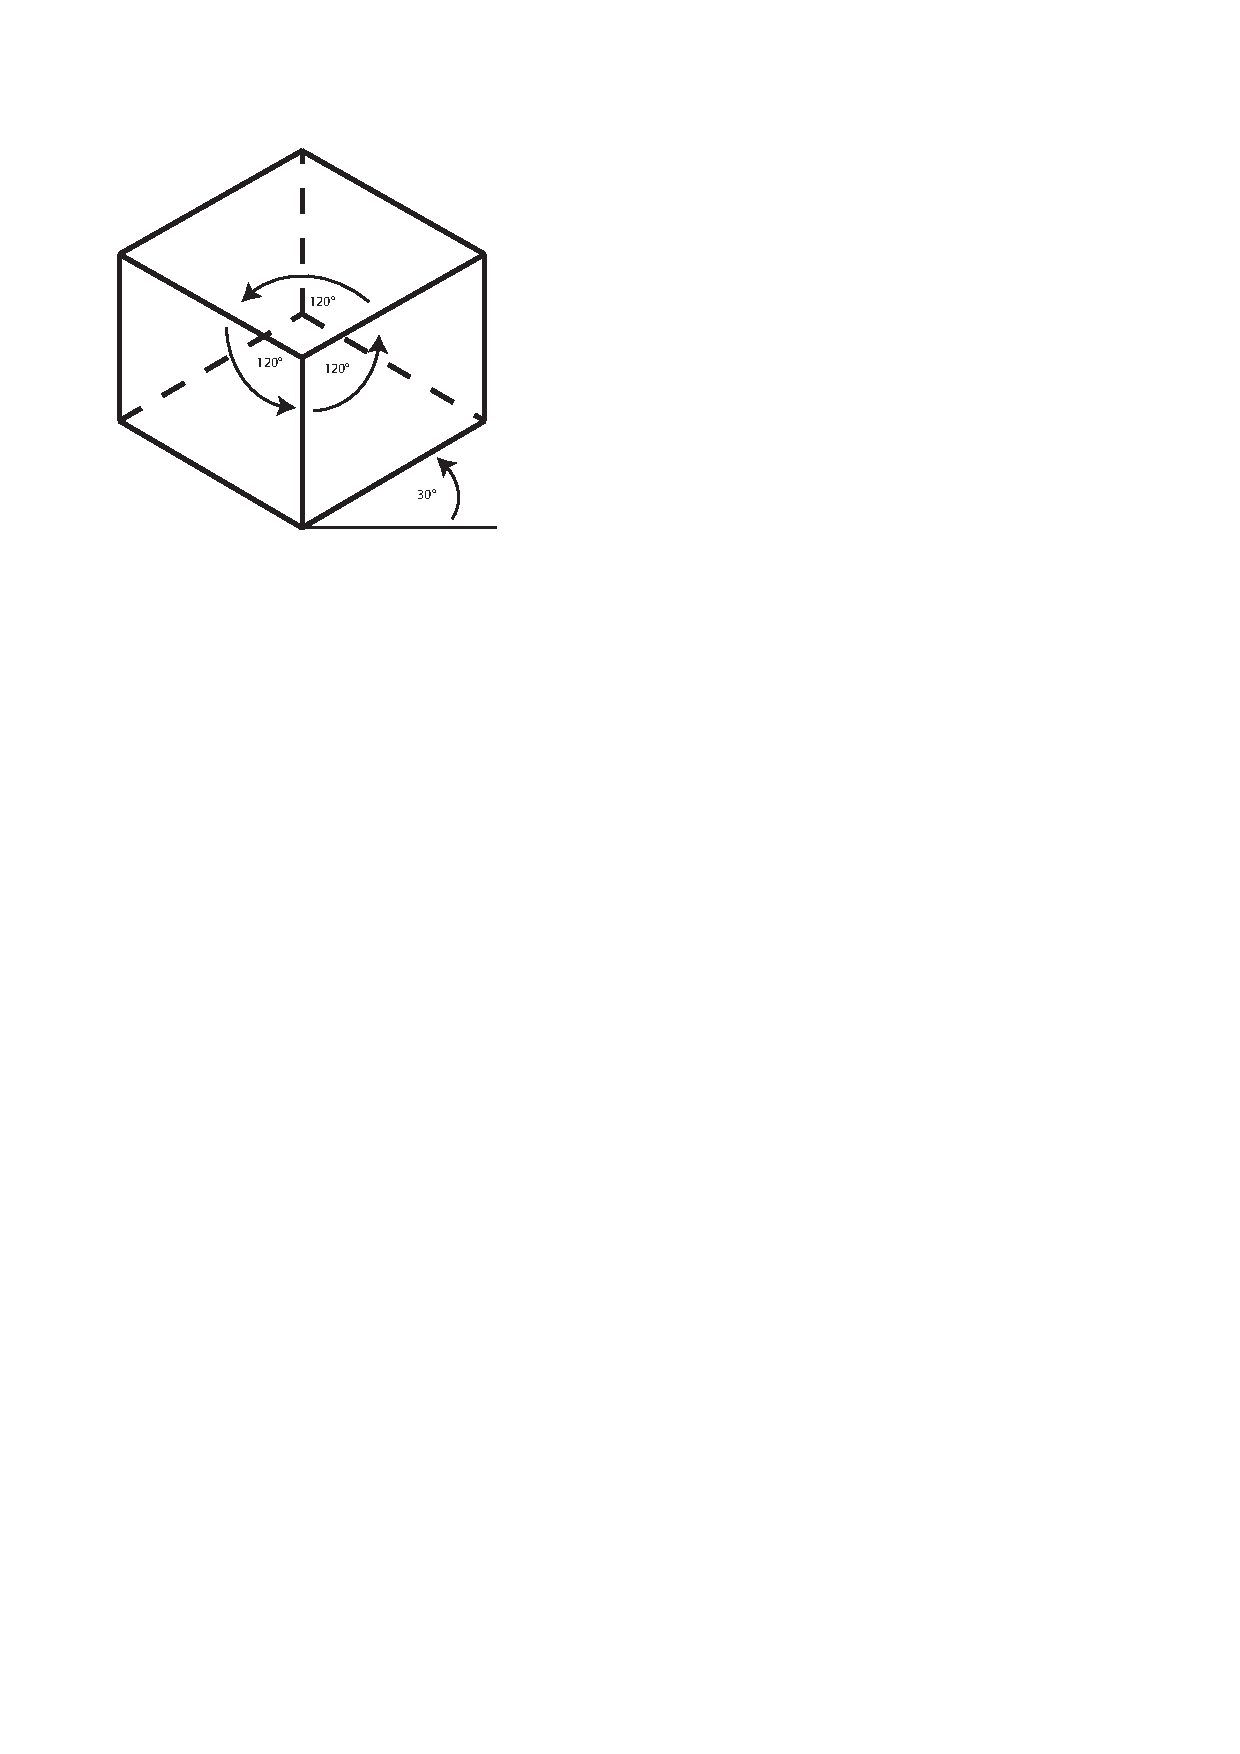
\includegraphics[clip=true,trim=0 205mm 100mm 20mm]{thesis-isobox}
	\caption{Isometric projection}
	\label{isometric}
\end{figure}

\subsection{Isometric camera}
The camera is top down, but tilted by 45 degrees in both directions. The diagonals therefore should be at 30 degrees, but due to the irregular aliasing of these diagonals on the bitmap grid the practical approach is slightly different. Figure \ref{isoangle} shows the problematic bitmap grid as well as the solution. The image is rotated by 45 degrees and then the aspect ratio is changed to 2:1. The result are regular 2pixel stairs forming diagonals in about 26.565 degrees\footnote{\begin{math}\arctan \frac{1}{2} \approx 26.565\si{\degree}\end{math}}. The side effect of this change is complete elimination of trigonometry from the projection mathematics further improving the rendering performance.

\begin{figure}[h]
	\centering
	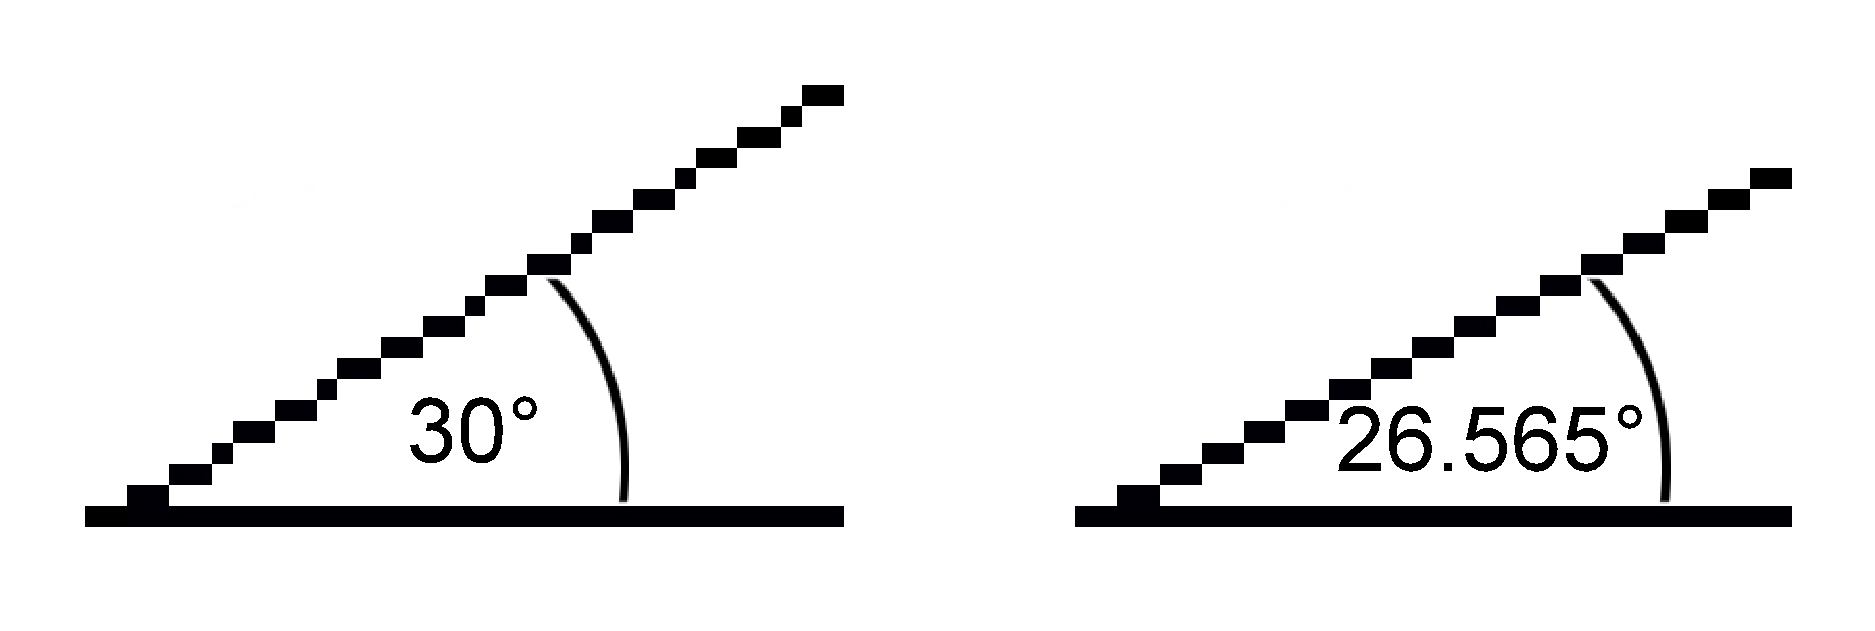
\includegraphics[width=0.7\textwidth]{thesis-angles}
	\caption{Isometric projection angle}
	\label{isoangle}
\end{figure}

\subsection{Example games, brief history}
The first game using isometric graphics was Zaxxon released by SEGA in 1982\cite{zaxxon} (see Figure \ref{zaxxon}). This new approach allowed to display 3D scene without the need for hardware accelerated 3D rendering. The same graphic style was later used in many other games, especially genres where the player overviews the scene from the top. \emph{Dune II} released in 1992\cite{dune2} used direct top-down camera. To improve the visual appeal, \emph{Warcraft: Orcs \& Humans} released two years later\cite{blizzardlegacy} tilted the camera slightly in one direction. Later games in the strategy genre\footnote{1990s classics including turn-based strategy \emph{Civilization II}\cite{civ2}, real-time strategy \emph{Age of Empires}\cite{ageofempires} and business simulator \emph{Transport Tycoon Deluxe}\cite{ttd}} fully adapted the isometric projection. These strategies often divided the map to regular tiles that limited the player actions but made collision detection and other game mechanics very simple. This design outlived the slow hardware with no graphic acceleration and is still popular both among independent developers with limited resources and in environments where hardware acceleration is not granted\footnote{Typically browser games discussed later.}. When 3D acceleration became affordable, focus of game development shifted to full 3D rendering. Although the player could be given full control of the camera, many games lock the camera in the same angle as is the isometric camera in order to avoid player confusion. Provided combination of realistic look of 3D rendered scene with perspective, shadows etc. and a clear overview of the scene defined by the isometric camera angle has proven to be optimal for wide array of games. Prime example be professionally played \emph{Starcraft 2}\cite{sc2} that does allow camera rotation, but the camera automatically returns to the original position soon afterwards.

\begin{figure}[h]
	\centering
	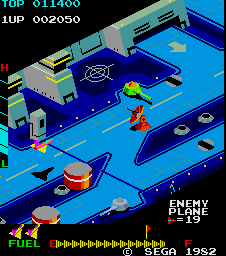
\includegraphics{zaxxon}
	\caption{Isometric graphics in original arcade version of Zaxxon\cite{zaxxon}}
	\label{zaxxon}
\end{figure}

\section{Web graphics and HTML5}
Web applications on the client side can rely only on the browser application and its capabilities. No middleware directly accessing hardware is guaranteed. Therefore the browser games\footnote{Games played on a web page displayed in the browser.} draw graphics to some element in the HTML page. Prior to the version 5 of the HTML standard, the games almost exclusively used Flash and required the client browser to have Adobe Flash Player plug-in installed\cite{flashplayer}. With the broad adoption of HTML5, new options presented themselves. Two new elements to display graphics allow to stop making any assumptions about the client other than whether it supports HTML5.

\subsection{Canvas, usage in games}
The \texttt{canvas} element is very similar to the canvas objects in other programming environments\footnote{E.g. classes \texttt{System.Windows.Controls.Canvas} in .NET framework\cite{net_canvas} or \texttt{java.awt.Canvas} in the Java platform\cite{java_canvas}}. It allows to directly draw to the canvas bitmap using JavaScript functions. Even though this approach is straight forward, some disadvantages arise when applied. Most noticeable is that when an object is being changed, everything that even partially covers it has to be re-drawn as well even if it stays unchanged on its own. Furthermore when drawing several objects that appear behind and in front of each other, these need to be carefully drawn in a correct order so the overlaps are correct and the illusion of space remains unbroken.

Due to the similarity to other environments there is already large variety of game engines implemented on the \texttt{canvas} element. Used underlying element is often reflected in the engine name\footnote{E.g. \emph{Canvace}\cite{canvace} or \emph{Canvas Engine}\cite{canvasengine}}, but other take \texttt{canvas} usage as a matter of course\footnote{E.g. \emph{enchant.js}\cite{enchantjs} or proprietary \emph{Isogenic Game Engine}\cite{isogenic}}.

\subsection{SVG}
The \texttt{svg} element is very different as it displays given SVG\footnote{Scalable Vector Graphics}, a vector image described in a markup language of the same name. It can also be dynamically manipulated with JavaScript, but the approach is fundamentally different. Elements are added to the DOM\footnote{Document Object Model} as if only standard HTML was used. Instead of redrawing the whole image or a part of screen, individual objects can be added, removed or changed. This makes for example an animation of an object much more straight forward. User interaction handling is easier as well since the event handlers can be hooked onto the elements representing the objects.

Even though browsers used to support static SVG for a long time, not until HTML5 did they support dynamic in-line SVG\cite{w3_html5}. This is now available with the previously mentioned element. Since rendering the markup language is much more complicated than simple dumping the canvas bitmap on the screen, the browser support is delayed and also more sensitive to performance problems. Drawing to the canvas may take a lot of JavaScript execution time, but in the end the display of the element takes amount of time only effected by the size of the canvas, not complexity of its content. Creating large SVG will take similar time, but then rendering it on the screen will take browser another time.

\chapter{Suggested solution / design}
\label{solution}
As it was discussed earlier, \texttt{canvas} based engines for browser games are quite common. Why is that there are no game engines based on \texttt{svg}? W3Schools in a chapter about HTML5 \texttt{svg} element warn that it, unlike the \texttt{canvas} element, is not suitable for game applications\cite{html5svg}. However is it possible to use an inline SVG to draw game graphics instead of the standard canvas approach? As proven by a demo build using Raphaël\footnote{An SVG manipulation library discussed later.}, at least a small game with simple graphics actually can be done\cite{raphaelfpsdemo}. With the event handling support, SVG should be even more suitable and furthermore manipulation with specific objects in a drawn scene should make the subsequent scene updates much easier.

The proposed idea is to make an attempt to create such engine. An engine that will be able to request data that describe area actually on screen, retrieved data will transform to their visual representation and render to the \texttt{svg} element. Of course all of this and the user interaction handling needs to be separated from the actual implementation for the engine to be generally usable by different end applications. To keep the scope focused enough so the implementation can provide some actually helpful functionality for the end application developer rather than just another abstraction layer over the SVG DOM, the engine shall be limited to render isometric tile-based graphics that are, as discussed earlier, still popular among both developers and players. This limitation allows the implementation to encapsulate all logic regarding isometric coordinate transformation.

\section{Data retrieval}
\label{datadesign}
Although in case of a single-player game\footnote{Game for only one player with no interaction with other people playing the same game.} the data can be completely generated and stored on the client instance, remote data retrieval needs to be supported as well. Furthermore since even single-player games are likely to store level map data in some common storage, the remote data access is expected to be prevalent use in eventual implementation usages. To keep the data transfer down, the data provider\footnote{Hereinafter referred to as the server.} is given an option to decide either to send full data matrix of requested area in the response or send only data of the tiles that changed since last request if the matrix of actually useful data would be too sparse. The former approach needs less data per tile since only the coordinates of a top left corner of the requested area needs to be included in the response since all other can be calculated from the response data. On the other hand the latter approach needs coordinates for each tile. Of course the efficiency of both ways depends on many other things. How thick or thin the client is hence whether the server keeps track of individual client request history. The tile data size to the two-integer coordinates ratio is also important as well as the volatility of the map data. Nevertheless both approaches find its use and the engine has to be able to process data presented in both formats.

The tile data record may contain more information than it is necessary to deduce the tile visual representation hence only a subset of this data record should be passed to the general map data requests to further lower the bandwidth usage. Then there must be a way to retrieve the rest of the tile data record for game logic purposes though. To provide this channel, engine has to implement a full data request for a tile involved in advanced operations.

\section{Sprites}
The standard way of making 2D games is to draw small images of objects and then compose the scene using these images. This way the object can be animated easily by replacing said image with next animation frame image. For performance reasons all these sprites are compiled to a single image called sprite-sheet.\cite{pagella} The graphics engine needs to be able to draw a sub-selection of the sprite-sheet image. When working with HTML5 \texttt{canvas} element, JavaScript function \texttt{CanvasRenderingContext2D.drawImage(img, sx, sy, swidth, sheight, x, y, width, height)} does exactly that\cite{canvasdrawimage}. First set of coordinates and dimensions determines which part of the source image will be drawn. Second set of coordinates and dimensions then determines the target location on the canvas.

When using SVG, no such a straightforward and convenient way is available. To display a section of an image, one needs to create a pattern from the image and position it using a negative coordinates. The pattern must use \emph{objectBoundingBox} units so it doesn't shrink the whole sprite-sheet in the target element. Then an SVG element (usually polygon) using this pattern can display desired selection of an image. The limitation of this approach is that all elements using the same pattern will have synchronous animation, what usually doesn't look too organic in the result. On the other hand it nicely emulates the early 90s era of gaming.

The more natural approach for \texttt{svg} would be having sprite-sheet defined as a separate SVG file containing vector sprites defined by SVG markup. Although this is certainly possible, vector graphics are not as widely used as bitmaps in the game development since creation of detailed vector assets is more complicated compared to the bitmaps.

Beside \texttt{canvas} the SVG also allows to use animated GIFs\footnote{Graphics Interchange Format is an image format that allows to contain a series of images that are displayed in sequence to show an animation\cite{gifstandard}.} as sprites. The creation of sprites or even sprite-sheets this way is more complicated. However when using sprites that are already animated, execution time needed to animate static tiles can be saved. The amount of saved time of course depends on the browser implementation and its support of said GIFs. In some cases this may even yield worse result than using static image formats.

\chapter{Used technologies}
\label{tech}

\section{Engine}
The graphics engine is being run on the client and hence all technologies used in it are based around JavaScript.

\subsection{Browser support of HTML5 SVG element}
HTML5's \texttt{svg} element as such is well supported by modern browsers\cite{html5svg}, but there are some difficulties with the implementation details in different browsers. A striking example be Internet Explorer that entirely lacks support of \texttt{foreignObject} SVG element that normally allows to nest HTML in the SVG image\cite{ieforeignobject}.

\subsection{SVG manipulation JavaScript libraries}
The contents of the \texttt{svg} element can be manipulated directly via JavaScript, but like regular HTML DOM manipulation, it is laborious and ends up with lots of repetitive code. To eliminate this drawback there are several JavaScript libraries that provide abstraction layer over the SVG markup. Most of them are open source.

A pioneer among these libraries is \emph{Raphaël}. The projects puts emphasis on wide browser support including archaic Internet Explorer version 6.0 \cite{raphael}.

\emph{Raphaël}'s rewrite, \emph{Snap.svg} is not held back by compatibility to obsolete browsers and so it can support features like masking, clipping, patterns, full gradients and groups\cite{snap}. Snap.svg is quite popular among front-end developers who typically create animation based on static SVG for web sites\cite{snapusage}. When working with SVG elements and their attributes are represented as string values. This may be perfect for mentioned application, but when creating all of the content dynamically, this involves a lot of string concatenation in the end, which is far from ideal in the intended use.

Next library called simply \emph{svg.js} takes more object oriented approach\cite{svgjs}, that is more suitable for this project. The project is modularized so for a production environment can be built with only the functionality that is really used to decrease script size. There are also quite a few additional modules providing extra functionality that might prove useful.

Another popular project called \emph{D3.js} does not limit its scope to SVG and approaches the DOM manipulation in a similar manner to \emph{jQuery}\cite{d3js}. Emphasis on querying the DOM, that is very performance demanding once the DOM has a large amount of elements, makes this project not suitable as well.

There are of course other libraries, but since the game developer using the engine will have to work with given SVG manipulation library to some extent, commonly used library with good documentation may make his use of the engine much easier. All considered, the \emph{svg.js} project was selected to serve as a SVG markup markup manipulation API.

\subsection{General utility JavaScript libraries}
\label{jslibs}
Other general purpose JavaScript libraries are used to keep the actual engine code clean and readable. Like the previously discussed libraries, these are open source as well and use non-restrictive licenses.

To help manage the JavaScript application structure, a library allowing to define modules and dependencies between them called \emph{require.js} is used. During execution on the client it makes sure all files containing required modules are loaded prior to their usage. \cite{requirejs} This approach eliminates many flaws of JavaScript as a language, particularly declaration scope confusion, possible redeclaration of variables and dependency on functions or variables that may not be declared yet.

Some very limited HTML manipulation is simplified using \emph{jQuery} library. Since the engine does not work with HTML out of the \texttt{svg} element the usage is rather minimal, mostly to access element properties in a unified fashion\footnote{Even something as simple as getting element's actual width can be quite laborious to get working across browsers without \emph{jQuery}.}. Since the display of game scene can generate quite a lot of elements, querying them, the main point of \emph{jQuery}\cite{jquery}, has to be done with performance in mind.

Automatic tests of the engine API are written using the \emph{Jasmine} framework. It allows to define test cases and expected behaviour\cite{jasmine}. Out of the box can these tests be run in the browser like the engine itself. Using the \emph{Karma} test runner the tests also can be integrated to the \emph{maven}\footnote{Maven is a build automation tool\cite{maven} used in this project mostly due to the demo back-end written in Java.} build process\cite{karma}.

\section{Other technologies used in the demo game}
The demo application created to demonstrate capabilities of the engine combines it with other technologies just like real world application would. Other application may change completely different set of dependencies, therefore the ones used in the demo application in no way bound to the actual engine.

\subsection{JavaScript objects provided by browsers}
Since the engine itself is abstracted from actual data source and format, the browser support for network communication and serialization is not needed until the specific game implementation.

For obtaining data from the server uses the demo application \texttt{XmlHttpRequest}, a JavaScript object widely supported by browsers\cite{xhr}. It allows to create an asynchronous HTTP request with a callback when the response is obtained.

To parse the JSON\footnote{JavaScript Object Notation data format} responses to a JavaScript object is used the \texttt{JSON} JavaScript object specified by ECMAScript 5.1 and also supported by modern browsers\cite{json}.

\subsection{RESTEasy}
RESTEasy is a JBoss project allowing to create a web service with parametrized URLs mapped to methods\cite{resteasy}. This service can very easily  provide RESTful\footnote{RESTful service meets all requirements defined by Representational State Transfer architecture, that is mainly unified access to creation, reading, update and deletion of provided resource\cite{fielding}.} management API, hence the project name. Jackson JAX-RS providers\cite{jackson} are used instead of the default JSON serializer to allow the service return custom Java objects with no additional annotations serialized to JSON. This framework was selected due to the simplicity of creating a service that provides access to the pseudo randomly generated data model of the demo application.

\subsection{AppEngine API}
Google App Engine is a cloud hosting service provided by Google. The engine demo application was hosted on this service for demonstration purposes and so the project had to contain piece of appropriate configuration. With generously limited bandwidth is the service free of charge. \cite{appengine}

\chapter{Implementation}
\label{implementation}
Important factor of the engine implementation is reusability that requires abstraction of all details of any specific game. Anything that would lead to these specifics is delegated to objects providing the specific game implementation via calling their interfaces. Figure \ref{classdiagram} shows dependencies among the engine JavaScript modules as well as the dependency to the external implementation of a specific game.

\begin{figure}[h]
	\centering
	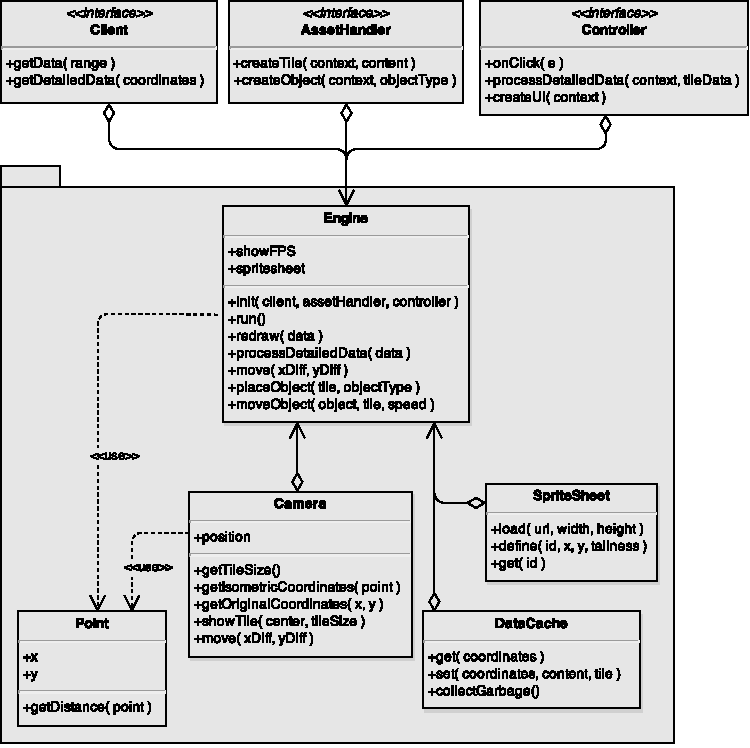
\includegraphics[width=\textwidth]{thesis-classdiagram}
	\caption{Diagram of the JavaScript modules}
	\label{classdiagram}
\end{figure}

For the purposes of the engine, the game implementation is divided to three interfaces, responsible for different aspects of the implementation. The \emph{Client} is supposed to bypass all server communication and \emph{AssetHandler} takes care of the data to visual representation translation. The last interface called \emph{Controller} is responsible for handling user interaction and game logic. Although the demo application implements each interface separately, nothing prevents the end application developer to implement all of them in a single object.

\section{Viewport population and data fetching}
As discussed in Chapter \ref{enginefunctionality}, the main responsibility of the engine is to draw the game scene to the screen. In case of tile-based games, this involves data that describe contents of all tiles to be even partially displayed in the current viewport\footnote{Viewport is a viewing region, in this case defined by a \texttt{div} element passed to the engine constructor.}. These data are periodically requested from the client object. An asynchronous callback on the engine then handles the response data, that can be continuous array of tile content values or if the client determines that few enough tiles changed, only content and coordinates of these changed tiles can be returned. This may save data traffic when repeatedly requesting updates of the same area as discussed in Chapter \ref{datadesign}.

The client--engine interaction could have been implemented in a push manner, but then would the client have to take responsibility for the game update loop. Since the game update loop is clearly responsibility of the game engine\cite{gregory}, engine is -- in configurable intervals -- polling the client for data updates.

Due to the isometric projection employed in the rendering, the range of tiles needed to populate the whole screen cannot be trivially defined. Figure \ref{isodata} shows the minimum amount of isometric tiles needed to cover a rectangular viewport. The dark grey tiles are not fully in the viewport, but still need to be rendered. To keep the data request simple and small, the white tiles are requested as well. Therefore the request may contain only of a top-left corner coordinates and then either width and height of the requested area or bottom-right coordinates. These options are mostly equivalent and for the engine implementation was chosen the latter one.

\begin{figure}[h]
	\centering
	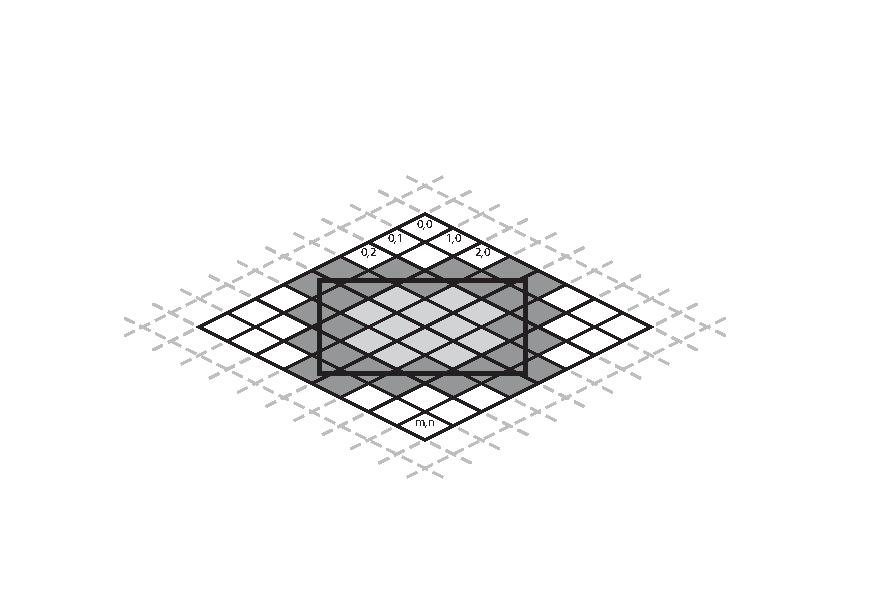
\includegraphics[clip=true,trim=20mm 17mm 20mm 23mm]{thesis-isodata}
	\caption{Data needed to fill a rectangular viewport}
	\label{isodata}
\end{figure}

\subsection{Data caching}
When the player moves around the map, server is requested for data on different locations. To make the player experience smoother, previously obtained data can be stored within the engine and if the player moves to the location of these data, potentially out-of-date tiles can be displayed meanwhile the new data is obtained. This way can be also utilized excessive data, discussed earlier, obtained with each response.

Storing data on the client involves a couple intricacies. These are connected to the behaviour of the JavaScript array object and its low level implementation. The problematic part is that only non negative integer indexes are supported by the array\cite{ecma}. Everything else -- be it negative integers, floating point numbers or straight up strings -- falls back to the property indexer. That is not only much slower than the array indexer, but also requires specific iteration. The tile coordinates are integers, but from the $(0,0)$ centre spread to all four directions, making half of them negative. Fortunately this can be eliminated by a simple transformation of the coordinates prior to the storage. Using the function declared in Figure \ref{indextransformation} the negative indexes are interspersed with the positive ones and the zero in the same manner a Turing machine with two way infinite tape can be simulated.

\begin{figure}[h]
\centering
\begin{math}
f(x) = 
\left\{
	\begin{array}{ll}
		2x  & \mbox{if } x \geq 0\\
		-2x - 1 & \mbox{if } x < 0
	\end{array}
\right.
\end{math}
\caption{Index transformation function}
\label{indextransformation}
\end{figure}

Array in JavaScript is natively sparse, therefore missing items take up close to no memory\cite{javascriptarray}. However collecting all obtained data without a thought is out of question since as a wise man said, ``a cache with a bad policy is another name for a memory leak''\cite{chen}. All obtained data can be cached as long as they are deleted at some point. The data cache implementation used in the engine uses to two-dimensional arrays to store tile data. Once is the first filled to a given limit, the second is filled instead and reading tries the current array first and if it fails, falls back to the older array. Once both arrays are filled to the given limit, older is deleted and serves as an empty current array. This mechanism is not very sophisticated, but does the job well enough.

\subsection{Isometric transformation}
All functionality linked to the isometric projection is encapsulated in the \emph{Camera} object implemented as a part of the engine. The transformation of orthogonal coordinates to the isometric ones defined in Figure \ref{isotransformation} needs to be modified to take into consideration also the fact that the data coordinates is in virtual tile units while the isometric coordinates used on screen need to be in pixels\cite{pagella}. Since the tile size in pixels is known, this can be achieved with a simple multiplication. Another necessary modification is to centre the whole transformed image to the screen by subtracting a half screen size offset.

\begin{figure}[h]
	\centering
	\begin{math}
		\begin{array}{lcl}
			isoX(x,y)&=&\frac{x - y}{2} \\\\
			isoY(x,y)&=&\frac{x + y}{2}
		\end{array}
	\end{math}
	\caption{Isometric coordinates transformation}
	\label{isotransformation}
\end{figure}

\section{Object stacking and verticality}
Just like when working with the full 3D projection, objects that are further away need to be hidden behind objects closer to the camera and objects that are on top need to hide objects beneath them. Otherwise the perception of space would be completely ruined. When working with a \texttt{canvas} element this needs to be handled by properly ordering all objects to be rendered so the objects in the foreground are drawn last and cover anything drawn prior to them before the actual rendering starts. When also considering the elevation of each element, this may become quite a complex operation. 

Fortunately a DOM manipulation -- be it SVG or standard HTML -- allows different approach. Standard DOM element function \texttt{insertBefore} allows to add element to a specified place in the element collection\cite{insertbefore}. Since the elements are rendered in the order in what they appear in this collection of siblings, the last remaining problem is to find where in this collection should the new element be placed. As long as a position in the map is stored with each tile element and the underlying tile stored with each object placed on that tile, the place where new element will hide everything that is behind while being covered with everything that is actually in front of it can be found. The indicator used in the engine implementation is a sum of both coordinates for it correlates with the y coordinate of isometric projection as is apparent in Figure \ref{isotransformation}. If all elements are added using this procedure, the collection is naturally ordered in the same manner as in the \texttt{canvas} case. It is also worth to notice that objects capable of position change need to be moved in the element collection during the movement. Otherwise an object that was correctly covering another object may end up still covering it even though it should not anymore. Figure \ref{movement} shows proper ordering change during a movement of sample objects, in this case a train car.

\begin{figure}[h]
	\centering
	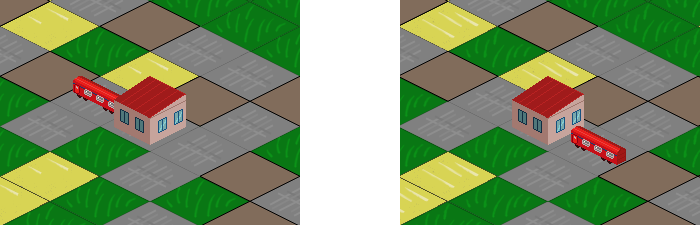
\includegraphics[width=\textwidth]{thesis-movement}
	\caption{Object movement handled by the engine}
	\label{movement}
\end{figure}

Objects elevated by either standing on something or flying in space need to handled extra in the isometric projection. Their altitude needs to be reflected in the final coordinates by a y-coordinate decrease. The engine calculates the amount of this decrease as a sum of heights all objects that are beneath given object on the same tile. Stacking objects on top of each other is shown on Figure \ref{stacking}.

\begin{figure}[h]
	\centering
	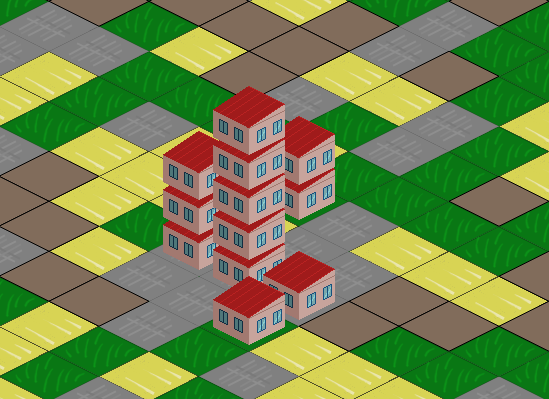
\includegraphics[width=\textwidth]{thesis-stacking}
	\caption{Object stacking handled by the engine}
	\label{stacking}
\end{figure}

\section{Asset declaration}
Whenever the engine needs to create something with visual representation, interface referred to as the asset handler is consulted. The asset handler functions are passed the SVG context in a parameter and are expected to create an SVG element according to the object type or content passed in other parameter. The engine then makes sure the result is added to appropriate place in the DOM and positioned to fit a location in the isometric projection.

This would cover the necessary engine functionality, but one further one more thing is implemented to make end user's life easier. When creating the element to visualize some data, the visual representation needs to be obtained from somewhere. To manage these in a form of bitmap sprites, an object called \emph{SpriteSheet} is made available. During the initialization of the game, one or more images can be loaded to memory and these or their parts can be declared as static or animated sprites. Each sprite is given an identifier so it can be later easily retrieved and used during the object creation. The sprite declaration needs to know the position of the sprite in the potentially larger sprite-sheet and optionally also the number of animation frames and the speed of the animation, or to be more precise the delay after each animation frame. Figure \ref{spritesheet} shows a sample sprite-sheet with three sprites, first is a desert with five animation frames, second is grass with only three animation frames and the last is static concrete with no animation. Usage of this sprite-sheet can be seen on the background of Figures \ref{stacking} and \ref{movement}. When the input image is an animated GIF, no animation needs to be declared with the sprites since it is performed by the browser, not by DOM manipulation caused by the engine.

\begin{figure}[h]
	\centering
	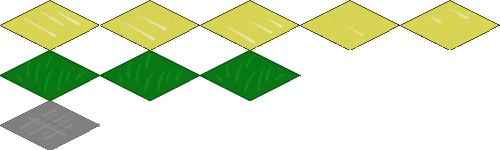
\includegraphics[width=\textwidth]{thesis-spritesheet}
	\caption{Sample sprite-sheet}
	\label{spritesheet}
\end{figure}

The \emph{SpriteSheet} is just an optional tool that can be ignored if the end application does not use bitmap sprites. In that case the SVG context is fully sufficient for the developer to create anything they may need.

\section{Update loop}
Even though the user interaction can be handled by asynchronous calls, a game engine still needs an ``infinite'' loop\footnote{A loop running for the whole duration of the game.} to update the game state according to external powers, game rules and to handle animations. The update loop can be implemented basically in two ways in JavaScript. The straight forward way would be to set interval and in the callback handle the game update. However using native interval is deprecated since the introduction of the \texttt{requestAnimationFrame} function\cite{raf}, the latter and better way. The scheduled interval cannot be synchronized with the browser update frequency and usually leads to unnecessary updates, especially when the browser window is not visible\cite{animationtiming}. Using \texttt{requestAnimationFrame} the update callback obtains a time stamp of the moment when the update was executed and can be compared with the same information obtained by previous update to calculate refresh rate or evaluate the necessity of server polling or sprite animation frame change. Since the engine needs a continuous loop, every update method needs to queue another animation frame request\cite{raf}. All of this is encapsulated in the \emph{Engine} object and everything the game needs to do after it is initialized is to call the \texttt{run} method.

\section{User interaction}
Handling the user interaction is delegated to the \emph{Controller} object serving as one of the game implementation interfaces. Controller is responsible for user interface creation as well as handling mouse and keyboard events. The engine attaches controller's \texttt{onClick} function to each tile created to make this easier. Keyboard handling can be implemented in the controller and does not require any support from the engine.

To obtain additional data, controller can entirely bypass the engine and call client directly. The result of detailed data request discussed in Chapter \ref{datadesign} is passed to the controller anyway since the graphics engine does not need these additional data for of its functionality.

To demonstrate the engine capabilities implements the demo application a couple of sample objects that the user can perform various actions with. The train car can be placed and moved. The building can be placed and then serve as a platform for more objects to be placed on. Both can be seen on Figure \ref{movement}. Even though so few restrictions given to the actions make little sense for a real game, actual game logic in the demo controller would be counterproductive only obscuring the engine usage.

\chapter{Testing and measurement}
\label{testing}
Testing JavaScript has its specifics, mainly due to the strong dependency to client web browser. Even though many standards were defined in an attempt to unify the browser behaviour, the actual implementations adopt the standards slowly and often deviate in seemingly minor details. Therefore the testing usually involves as many browsers as is expected to be commonly used among the target user base. One can be careful not to use anything unsupported by some of target browsers, but at the end of the day, running the application in all of the browsers still may discover some compatibility issues. Automation of this process may save quite a lot of time. 

\section{Automatic testing}
Part of the build process of the project containing the engine implementation are automatic tests. The expected behaviour of most of the implemented functionality is verified by running all of these tests by the end of each build to detect regression of bugs. The automatic tests can easily check API behaviour in extreme cases that may be very difficult to reach from the user interface. The \emph{Karma} runner discussed in Chapter \ref{jslibs} used to do the execution of tests defined in JavaScript can be configured to run the complete test suite in many supported browser environments, however usually only single environment is enough to discover discrepancies created by an incautious refactoring. 

\section{Performance in various browsers}
One of more likely reasons for the \texttt{svg} element to be inferior to the commonly used \texttt{canvas} element in regards to the game graphics could be insufficient performance when working with a scene rendered as a large amount of SVG elements. In extreme case this could make the \texttt{svg} element completely useless for more complex games. To test this concern, a performance evaluation of the final engine has been performed on various platforms available at the time.

\subsection{Basic test scenario}
The primary test scenario consisted of rendering an area of given size covered with pseudo random distribution of static and animated tiles. The area size used for majority of the cases was 1920 pixels by 1080 pixels, which is equal to the industry standard size of HD displays. Roughly a thousand tiles was needed to fill the area. Twice a second a server update was requested resulting in content update of fifty tiles. After initialization of the scene one minute was given to stabilize the frame-rate. Then a thousand objects\footnote{The building object visible in Figure \ref{stacking} was used for this scenario, but any other object could have been used.} was added one by one with one second delay after each addition. An average frame-rate over each of these second long intervals was recorded with the current number of added objects. All of this was scripted in a similar manner to the automatic tests. The scenario was designed this way to simulate the normal usage by a player of potential strategic game. By the end of the scenario execution, the screen would look like is shown at Figure \ref{performance-finish}. One execution of the scenario takes roughly 20 minutes regardless on the used hardware due to the delays. The machines used to run the performance tests were running Microsoft Windows 7 and during the tests also served to run the web server hosting the tested application and providing data updates.

\begin{figure}[h]
	\centering
	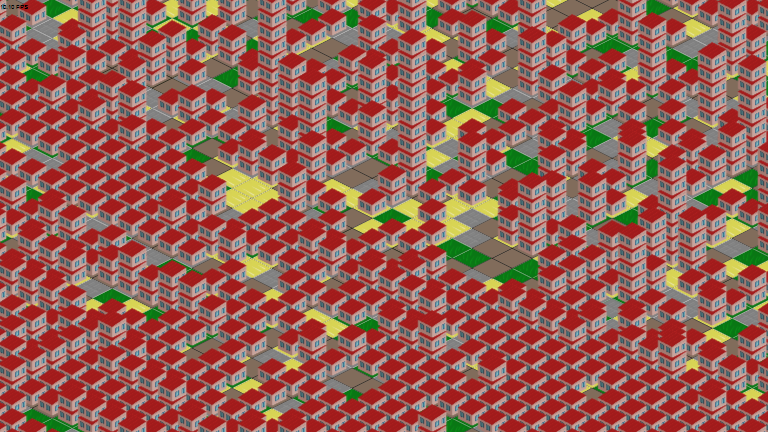
\includegraphics[width=\textwidth]{thesis-performance-finish}
	\caption{Screen depicting the end of the performance test scenario}
	\label{performance-finish}
\end{figure}

Described scenario was run in various currently relevant web browsers, including very common Google Chrome, Mozilla Firefox, Microsoft Internet Explorer, lately not very frequent Opera. As a curiosity also Firefox compiled with optimizations for 64bit systems called Waterfox\cite{waterfox} and recently announced Vivaldi available as a technical preview\cite{vivaldi}. The ideal frame-rate is at 60 FPS or only slightly bellow, but games are usually still playable down to 20 FPS\footnote{Depending on game genre -- games that require quick reactions require higher frame-rate to be played.}. Figure \ref{performance-basic} shows results across all the tested browsers. The striking similarity of top three lines can be explained by Chrome, Opera and Vivaldi sharing the same layout engine -- \emph{Blink} that is a fork of \emph{WebKIT}\cite{webkit}. Substantial drop in frame-rate can be noticed when the screen has been filled with more than 300 objects. At that point was the screen already completely cluttered with objects. Both Firefox and Waterfox showed very unstable and borderline usable frame-rate. The Internet Explorer proved useless with this much elements on screen.

\begin{figure}[h]
	\centering
	% GNUPLOT: LaTeX picture with Postscript
\begingroup
\newcommand{\ft}[0]{\footnotesize}
  \makeatletter
  \providecommand\color[2][]{%
    \GenericError{(gnuplot) \space\space\space\@spaces}{%
      Package color not loaded in conjunction with
      terminal option `colourtext'%
    }{See the gnuplot documentation for explanation.%
    }{Either use 'blacktext' in gnuplot or load the package
      color.sty in LaTeX.}%
    \renewcommand\color[2][]{}%
  }%
  \providecommand\includegraphics[2][]{%
    \GenericError{(gnuplot) \space\space\space\@spaces}{%
      Package graphicx or graphics not loaded%
    }{See the gnuplot documentation for explanation.%
    }{The gnuplot epslatex terminal needs graphicx.sty or graphics.sty.}%
    \renewcommand\includegraphics[2][]{}%
  }%
  \providecommand\rotatebox[2]{#2}%
  \@ifundefined{ifGPcolor}{%
    \newif\ifGPcolor
    \GPcolortrue
  }{}%
  \@ifundefined{ifGPblacktext}{%
    \newif\ifGPblacktext
    \GPblacktexttrue
  }{}%
  % define a \g@addto@macro without @ in the name:
  \let\gplgaddtomacro\g@addto@macro
  % define empty templates for all commands taking text:
  \gdef\gplbacktext{}%
  \gdef\gplfronttext{}%
  \makeatother
  \ifGPblacktext
    % no textcolor at all
    \def\colorrgb#1{}%
    \def\colorgray#1{}%
  \else
    % gray or color?
    \ifGPcolor
      \def\colorrgb#1{\color[rgb]{#1}}%
      \def\colorgray#1{\color[gray]{#1}}%
      \expandafter\def\csname LTw\endcsname{\color{white}}%
      \expandafter\def\csname LTb\endcsname{\color{black}}%
      \expandafter\def\csname LTa\endcsname{\color{black}}%
      \expandafter\def\csname LT0\endcsname{\color[rgb]{1,0,0}}%
      \expandafter\def\csname LT1\endcsname{\color[rgb]{0,1,0}}%
      \expandafter\def\csname LT2\endcsname{\color[rgb]{0,0,1}}%
      \expandafter\def\csname LT3\endcsname{\color[rgb]{1,0,1}}%
      \expandafter\def\csname LT4\endcsname{\color[rgb]{0,1,1}}%
      \expandafter\def\csname LT5\endcsname{\color[rgb]{1,1,0}}%
      \expandafter\def\csname LT6\endcsname{\color[rgb]{0,0,0}}%
      \expandafter\def\csname LT7\endcsname{\color[rgb]{1,0.3,0}}%
      \expandafter\def\csname LT8\endcsname{\color[rgb]{0.5,0.5,0.5}}%
    \else
      % gray
      \def\colorrgb#1{\color{black}}%
      \def\colorgray#1{\color[gray]{#1}}%
      \expandafter\def\csname LTw\endcsname{\color{white}}%
      \expandafter\def\csname LTb\endcsname{\color{black}}%
      \expandafter\def\csname LTa\endcsname{\color{black}}%
      \expandafter\def\csname LT0\endcsname{\color{black}}%
      \expandafter\def\csname LT1\endcsname{\color{black}}%
      \expandafter\def\csname LT2\endcsname{\color{black}}%
      \expandafter\def\csname LT3\endcsname{\color{black}}%
      \expandafter\def\csname LT4\endcsname{\color{black}}%
      \expandafter\def\csname LT5\endcsname{\color{black}}%
      \expandafter\def\csname LT6\endcsname{\color{black}}%
      \expandafter\def\csname LT7\endcsname{\color{black}}%
      \expandafter\def\csname LT8\endcsname{\color{black}}%
    \fi
  \fi
    \setlength{\unitlength}{0.0500bp}%
    \ifx\gptboxheight\undefined%
      \newlength{\gptboxheight}%
      \newlength{\gptboxwidth}%
      \newsavebox{\gptboxtext}%
    \fi%
    \setlength{\fboxrule}{0.5pt}%
    \setlength{\fboxsep}{1pt}%
\begin{picture}(7370.00,5668.00)%
    \gplgaddtomacro\gplbacktext{%
      \csname LTb\endcsname%
      \put(682,704){\makebox(0,0)[r]{\strut{}$0$}}%
      \put(682,1487){\makebox(0,0)[r]{\strut{}$10$}}%
      \put(682,2270){\makebox(0,0)[r]{\strut{}$20$}}%
      \put(682,3054){\makebox(0,0)[r]{\strut{}$30$}}%
      \put(682,3837){\makebox(0,0)[r]{\strut{}$40$}}%
      \put(682,4620){\makebox(0,0)[r]{\strut{}$50$}}%
      \put(682,5403){\makebox(0,0)[r]{\strut{}$60$}}%
      \put(814,484){\makebox(0,0){\strut{}$0$}}%
      \put(2046,484){\makebox(0,0){\strut{}$200$}}%
      \put(3278,484){\makebox(0,0){\strut{}$400$}}%
      \put(4509,484){\makebox(0,0){\strut{}$600$}}%
      \put(5741,484){\makebox(0,0){\strut{}$800$}}%
      \put(6973,484){\makebox(0,0){\strut{}$1000$}}%
    }%
    \gplgaddtomacro\gplfronttext{%
      \csname LTb\endcsname%
      \put(176,3053){\rotatebox{-270}{\makebox(0,0){\strut{}FPS}}}%
      \put(3893,154){\makebox(0,0){\strut{}Objects count}}%
      \csname LTb\endcsname%
      \put(5986,5230){\makebox(0,0)[r]{\strut{}Chrome 42.0}}%
      \csname LTb\endcsname%
      \put(5986,5010){\makebox(0,0)[r]{\strut{}Firefox 38.0}}%
      \csname LTb\endcsname%
      \put(5986,4790){\makebox(0,0)[r]{\strut{}Internet Explorer 11.0}}%
      \csname LTb\endcsname%
      \put(5986,4570){\makebox(0,0)[r]{\strut{}Opera 29.0}}%
      \csname LTb\endcsname%
      \put(5986,4350){\makebox(0,0)[r]{\strut{}Vivaldi 1.0}}%
      \csname LTb\endcsname%
      \put(5986,4130){\makebox(0,0)[r]{\strut{}Waterfox 38.0}}%
    }%
    \gplbacktext
    \put(0,0){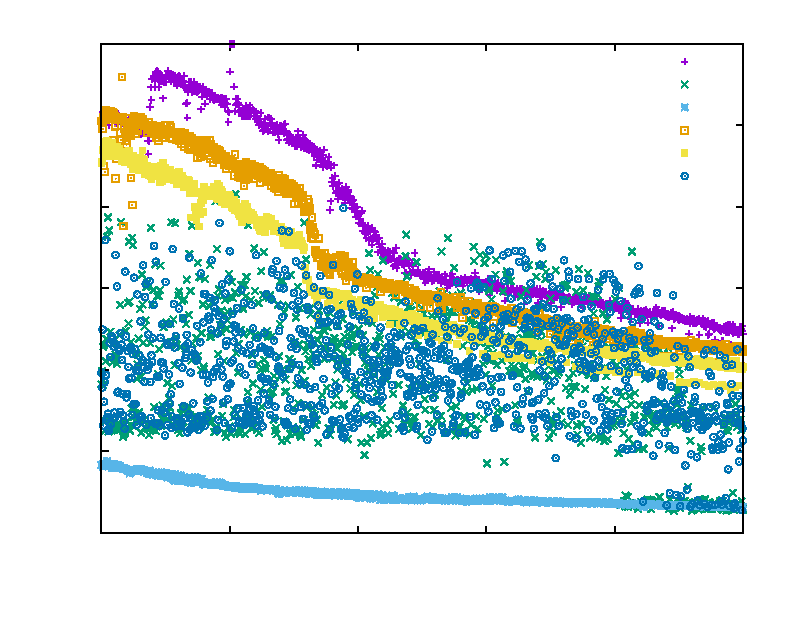
\includegraphics{thesis-performance-basic}}%
    \gplfronttext
  \end{picture}%
\endgroup

	\caption{Performance test results across browsers}
	\label{performance-basic}
\end{figure}

Worth notice is also the browser hardware usage CPU usage during the tests, all run on a 64bit desktop PC with 4core Intel Core i5 2500K CPU at 3.3~GHz and 8~GB of RAM. None of the browsers deviated by excessive memory usage. However the WebKIT based browsers spawning multiple processes that used around 60~\% of the CPU while Firefox steadily occupied only 30~\% of CPU and the abstemious Internet Explorer consumed only around a quarter of the CPU time.

\begin{figure}[h]
	\centering
	% GNUPLOT: LaTeX picture with Postscript
\begingroup
  \makeatletter
  \providecommand\color[2][]{%
    \GenericError{(gnuplot) \space\space\space\@spaces}{%
      Package color not loaded in conjunction with
      terminal option `colourtext'%
    }{See the gnuplot documentation for explanation.%
    }{Either use 'blacktext' in gnuplot or load the package
      color.sty in LaTeX.}%
    \renewcommand\color[2][]{}%
  }%
  \providecommand\includegraphics[2][]{%
    \GenericError{(gnuplot) \space\space\space\@spaces}{%
      Package graphicx or graphics not loaded%
    }{See the gnuplot documentation for explanation.%
    }{The gnuplot epslatex terminal needs graphicx.sty or graphics.sty.}%
    \renewcommand\includegraphics[2][]{}%
  }%
  \providecommand\rotatebox[2]{#2}%
  \@ifundefined{ifGPcolor}{%
    \newif\ifGPcolor
    \GPcolortrue
  }{}%
  \@ifundefined{ifGPblacktext}{%
    \newif\ifGPblacktext
    \GPblacktexttrue
  }{}%
  % define a \g@addto@macro without @ in the name:
  \let\gplgaddtomacro\g@addto@macro
  % define empty templates for all commands taking text:
  \gdef\gplbacktext{}%
  \gdef\gplfronttext{}%
  \makeatother
  \ifGPblacktext
    % no textcolor at all
    \def\colorrgb#1{}%
    \def\colorgray#1{}%
  \else
    % gray or color?
    \ifGPcolor
      \def\colorrgb#1{\color[rgb]{#1}}%
      \def\colorgray#1{\color[gray]{#1}}%
      \expandafter\def\csname LTw\endcsname{\color{white}}%
      \expandafter\def\csname LTb\endcsname{\color{black}}%
      \expandafter\def\csname LTa\endcsname{\color{black}}%
      \expandafter\def\csname LT0\endcsname{\color[rgb]{1,0,0}}%
      \expandafter\def\csname LT1\endcsname{\color[rgb]{0,1,0}}%
      \expandafter\def\csname LT2\endcsname{\color[rgb]{0,0,1}}%
      \expandafter\def\csname LT3\endcsname{\color[rgb]{1,0,1}}%
      \expandafter\def\csname LT4\endcsname{\color[rgb]{0,1,1}}%
      \expandafter\def\csname LT5\endcsname{\color[rgb]{1,1,0}}%
      \expandafter\def\csname LT6\endcsname{\color[rgb]{0,0,0}}%
      \expandafter\def\csname LT7\endcsname{\color[rgb]{1,0.3,0}}%
      \expandafter\def\csname LT8\endcsname{\color[rgb]{0.5,0.5,0.5}}%
    \else
      % gray
      \def\colorrgb#1{\color{black}}%
      \def\colorgray#1{\color[gray]{#1}}%
      \expandafter\def\csname LTw\endcsname{\color{white}}%
      \expandafter\def\csname LTb\endcsname{\color{black}}%
      \expandafter\def\csname LTa\endcsname{\color{black}}%
      \expandafter\def\csname LT0\endcsname{\color{black}}%
      \expandafter\def\csname LT1\endcsname{\color{black}}%
      \expandafter\def\csname LT2\endcsname{\color{black}}%
      \expandafter\def\csname LT3\endcsname{\color{black}}%
      \expandafter\def\csname LT4\endcsname{\color{black}}%
      \expandafter\def\csname LT5\endcsname{\color{black}}%
      \expandafter\def\csname LT6\endcsname{\color{black}}%
      \expandafter\def\csname LT7\endcsname{\color{black}}%
      \expandafter\def\csname LT8\endcsname{\color{black}}%
    \fi
  \fi
    \setlength{\unitlength}{0.0500bp}%
    \ifx\gptboxheight\undefined%
      \newlength{\gptboxheight}%
      \newlength{\gptboxwidth}%
      \newsavebox{\gptboxtext}%
    \fi%
    \setlength{\fboxrule}{0.5pt}%
    \setlength{\fboxsep}{1pt}%
\begin{picture}(7370.00,5668.00)%
    \gplgaddtomacro\gplbacktext{%
      \csname LTb\endcsname%
      \put(682,704){\makebox(0,0)[r]{\strut{}$0$}}%
      \put(682,1487){\makebox(0,0)[r]{\strut{}$10$}}%
      \put(682,2270){\makebox(0,0)[r]{\strut{}$20$}}%
      \put(682,3054){\makebox(0,0)[r]{\strut{}$30$}}%
      \put(682,3837){\makebox(0,0)[r]{\strut{}$40$}}%
      \put(682,4620){\makebox(0,0)[r]{\strut{}$50$}}%
      \put(682,5403){\makebox(0,0)[r]{\strut{}$60$}}%
      \put(814,484){\makebox(0,0){\strut{}$0$}}%
      \put(2046,484){\makebox(0,0){\strut{}$200$}}%
      \put(3278,484){\makebox(0,0){\strut{}$400$}}%
      \put(4509,484){\makebox(0,0){\strut{}$600$}}%
      \put(5741,484){\makebox(0,0){\strut{}$800$}}%
      \put(6973,484){\makebox(0,0){\strut{}$1000$}}%
    }%
    \gplgaddtomacro\gplfronttext{%
      \csname LTb\endcsname%
      \put(176,3053){\rotatebox{-270}{\makebox(0,0){\strut{}FPS}}}%
      \put(3893,154){\makebox(0,0){\strut{}Objects count}}%
      \csname LTb\endcsname%
      \put(5986,5230){\makebox(0,0)[r]{\strut{}Chrome 42.0}}%
      \csname LTb\endcsname%
      \put(5986,5010){\makebox(0,0)[r]{\strut{}Internet Explorer 11.0}}%
      \csname LTb\endcsname%
      \put(5986,4790){\makebox(0,0)[r]{\strut{}Firefox 38.0}}%
    }%
    \gplbacktext
    \put(0,0){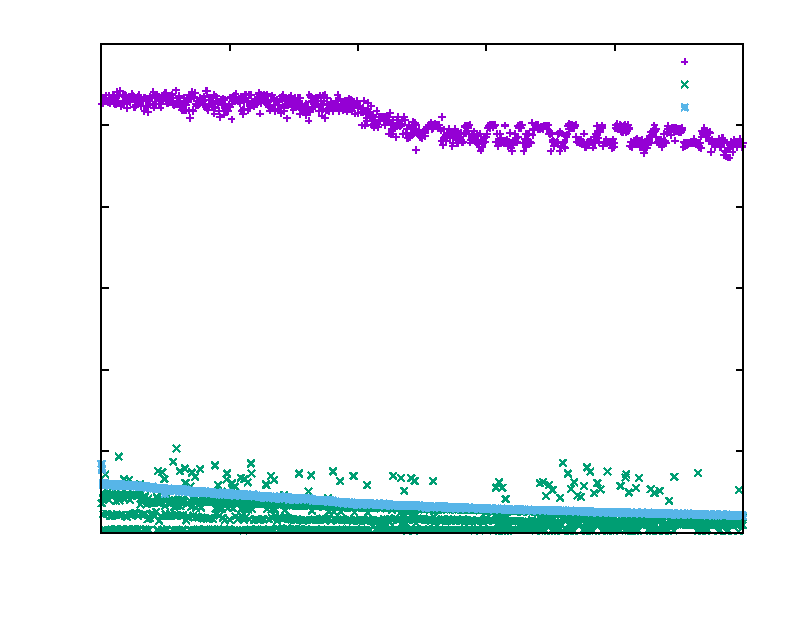
\includegraphics{thesis-performance-gif}}%
    \gplfronttext
  \end{picture}%
\endgroup

	\caption{Results of the second test featuring animated GIF sprites}
	\label{performance-gif}
\end{figure}

\subsection{Performance impact of animated GIF sprites}
Selected browsers were subjected to another test, using the same scenario but now using animated GIF sprites instead of handling the animation in the engine code. Since WebKIT based browsers proved to perform very similarly and there was no difference between Firefox and Waterfox either during the earlier tests, only Chrome, Firefox and Internet Explorer were subjected to the second test. Results are displayed in Figure \ref{performance-gif}. While the frame-rate drop after a certain amount of object has been added to the scene present with Chrome during the previous test was eliminated, earlier all over the place Firefox frame-rate fell just above the Internet Explorer level. These changes in the performance suggest that using standard sprites and letting the engine animate them in the JavaScript code would be in most cases a better option.

\subsection{Other performance influences}
To compare how the engine performance scales with other properties of the environment, two more tests were performed. The first tried the so far best performing browser on a PC with considerably older hardware. The second testing machine was a laptop with 4 GB of RAM and Intel Pentium Dual-Core T3400 at 2.16 GHz, however as the name suggests, with only 2 cores. Figure \ref{performance-hw} compares results of the previous machine and the slower laptop. Using the older hardware, Chrome manage to keep frame-rate only barely usable.

\begin{figure}[h]
	\centering
	% GNUPLOT: LaTeX picture with Postscript
\begingroup
  \makeatletter
  \providecommand\color[2][]{%
    \GenericError{(gnuplot) \space\space\space\@spaces}{%
      Package color not loaded in conjunction with
      terminal option `colourtext'%
    }{See the gnuplot documentation for explanation.%
    }{Either use 'blacktext' in gnuplot or load the package
      color.sty in LaTeX.}%
    \renewcommand\color[2][]{}%
  }%
  \providecommand\includegraphics[2][]{%
    \GenericError{(gnuplot) \space\space\space\@spaces}{%
      Package graphicx or graphics not loaded%
    }{See the gnuplot documentation for explanation.%
    }{The gnuplot epslatex terminal needs graphicx.sty or graphics.sty.}%
    \renewcommand\includegraphics[2][]{}%
  }%
  \providecommand\rotatebox[2]{#2}%
  \@ifundefined{ifGPcolor}{%
    \newif\ifGPcolor
    \GPcolortrue
  }{}%
  \@ifundefined{ifGPblacktext}{%
    \newif\ifGPblacktext
    \GPblacktexttrue
  }{}%
  % define a \g@addto@macro without @ in the name:
  \let\gplgaddtomacro\g@addto@macro
  % define empty templates for all commands taking text:
  \gdef\gplbacktext{}%
  \gdef\gplfronttext{}%
  \makeatother
  \ifGPblacktext
    % no textcolor at all
    \def\colorrgb#1{}%
    \def\colorgray#1{}%
  \else
    % gray or color?
    \ifGPcolor
      \def\colorrgb#1{\color[rgb]{#1}}%
      \def\colorgray#1{\color[gray]{#1}}%
      \expandafter\def\csname LTw\endcsname{\color{white}}%
      \expandafter\def\csname LTb\endcsname{\color{black}}%
      \expandafter\def\csname LTa\endcsname{\color{black}}%
      \expandafter\def\csname LT0\endcsname{\color[rgb]{1,0,0}}%
      \expandafter\def\csname LT1\endcsname{\color[rgb]{0,1,0}}%
      \expandafter\def\csname LT2\endcsname{\color[rgb]{0,0,1}}%
      \expandafter\def\csname LT3\endcsname{\color[rgb]{1,0,1}}%
      \expandafter\def\csname LT4\endcsname{\color[rgb]{0,1,1}}%
      \expandafter\def\csname LT5\endcsname{\color[rgb]{1,1,0}}%
      \expandafter\def\csname LT6\endcsname{\color[rgb]{0,0,0}}%
      \expandafter\def\csname LT7\endcsname{\color[rgb]{1,0.3,0}}%
      \expandafter\def\csname LT8\endcsname{\color[rgb]{0.5,0.5,0.5}}%
    \else
      % gray
      \def\colorrgb#1{\color{black}}%
      \def\colorgray#1{\color[gray]{#1}}%
      \expandafter\def\csname LTw\endcsname{\color{white}}%
      \expandafter\def\csname LTb\endcsname{\color{black}}%
      \expandafter\def\csname LTa\endcsname{\color{black}}%
      \expandafter\def\csname LT0\endcsname{\color{black}}%
      \expandafter\def\csname LT1\endcsname{\color{black}}%
      \expandafter\def\csname LT2\endcsname{\color{black}}%
      \expandafter\def\csname LT3\endcsname{\color{black}}%
      \expandafter\def\csname LT4\endcsname{\color{black}}%
      \expandafter\def\csname LT5\endcsname{\color{black}}%
      \expandafter\def\csname LT6\endcsname{\color{black}}%
      \expandafter\def\csname LT7\endcsname{\color{black}}%
      \expandafter\def\csname LT8\endcsname{\color{black}}%
    \fi
  \fi
    \setlength{\unitlength}{0.0500bp}%
    \ifx\gptboxheight\undefined%
      \newlength{\gptboxheight}%
      \newlength{\gptboxwidth}%
      \newsavebox{\gptboxtext}%
    \fi%
    \setlength{\fboxrule}{0.5pt}%
    \setlength{\fboxsep}{1pt}%
\begin{picture}(7370.00,5668.00)%
    \gplgaddtomacro\gplbacktext{%
      \csname LTb\endcsname%
      \put(682,704){\makebox(0,0)[r]{\strut{}$0$}}%
      \put(682,1487){\makebox(0,0)[r]{\strut{}$10$}}%
      \put(682,2270){\makebox(0,0)[r]{\strut{}$20$}}%
      \put(682,3054){\makebox(0,0)[r]{\strut{}$30$}}%
      \put(682,3837){\makebox(0,0)[r]{\strut{}$40$}}%
      \put(682,4620){\makebox(0,0)[r]{\strut{}$50$}}%
      \put(682,5403){\makebox(0,0)[r]{\strut{}$60$}}%
      \put(814,484){\makebox(0,0){\strut{}$0$}}%
      \put(2046,484){\makebox(0,0){\strut{}$200$}}%
      \put(3278,484){\makebox(0,0){\strut{}$400$}}%
      \put(4509,484){\makebox(0,0){\strut{}$600$}}%
      \put(5741,484){\makebox(0,0){\strut{}$800$}}%
      \put(6973,484){\makebox(0,0){\strut{}$1000$}}%
    }%
    \gplgaddtomacro\gplfronttext{%
      \csname LTb\endcsname%
      \put(176,3053){\rotatebox{-270}{\makebox(0,0){\strut{}FPS}}}%
      \put(3893,154){\makebox(0,0){\strut{}Objects count}}%
      \csname LTb\endcsname%
      \put(5986,5230){\makebox(0,0)[r]{\strut{}i5 2500K}}%
      \csname LTb\endcsname%
      \put(5986,5010){\makebox(0,0)[r]{\strut{}Pentium Dual-Core T3400}}%
    }%
    \gplbacktext
    \put(0,0){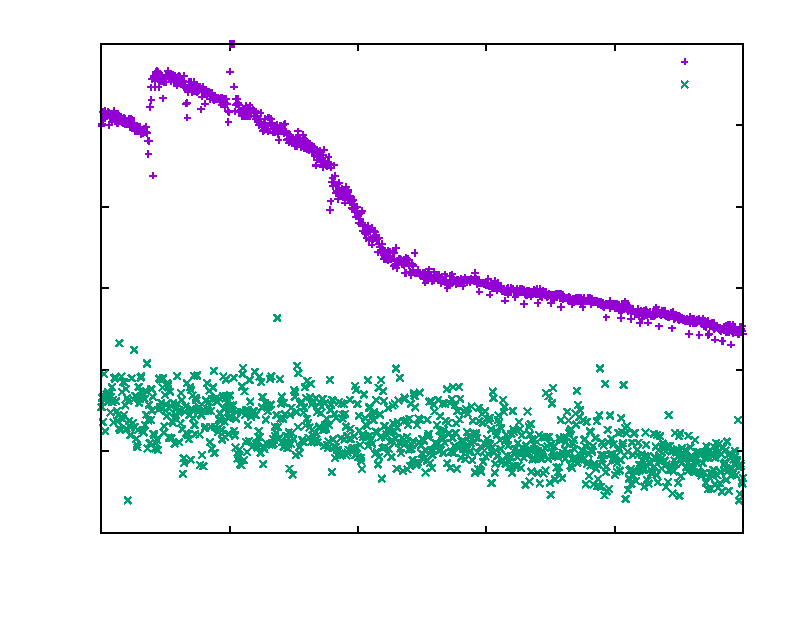
\includegraphics{thesis-performance-cpus}}%
    \gplfronttext
  \end{picture}%
\endgroup

	\caption{Hardware influence on the engine performance in Chrome 42.0}
	\label{performance-hw}
\end{figure}

Since the area used in all previous tests was quite large, even larger than the display of display used in previous tests, a smaller area was used in attempt to achieve better frame-rate by the overall slowest browser, Internet Explorer. Same scenario was used only with the area resolution halved in both directions, effectively making circa 250 tiles fill the screen instead of original thousand. Since the amount of objects added was kept the same, at the end of the scenario, the area was four times more cluttered by objects. As Figure \ref{performance-size} shows, for a managed Internet Explorer twice higher frame-rate until it got overwhelmed by the amount of objects added. At the end there was no difference caused by the smaller size of the rendered area.

\begin{figure}[h]
	\centering
	% GNUPLOT: LaTeX picture with Postscript
\begingroup
  \makeatletter
  \providecommand\color[2][]{%
    \GenericError{(gnuplot) \space\space\space\@spaces}{%
      Package color not loaded in conjunction with
      terminal option `colourtext'%
    }{See the gnuplot documentation for explanation.%
    }{Either use 'blacktext' in gnuplot or load the package
      color.sty in LaTeX.}%
    \renewcommand\color[2][]{}%
  }%
  \providecommand\includegraphics[2][]{%
    \GenericError{(gnuplot) \space\space\space\@spaces}{%
      Package graphicx or graphics not loaded%
    }{See the gnuplot documentation for explanation.%
    }{The gnuplot epslatex terminal needs graphicx.sty or graphics.sty.}%
    \renewcommand\includegraphics[2][]{}%
  }%
  \providecommand\rotatebox[2]{#2}%
  \@ifundefined{ifGPcolor}{%
    \newif\ifGPcolor
    \GPcolortrue
  }{}%
  \@ifundefined{ifGPblacktext}{%
    \newif\ifGPblacktext
    \GPblacktexttrue
  }{}%
  % define a \g@addto@macro without @ in the name:
  \let\gplgaddtomacro\g@addto@macro
  % define empty templates for all commands taking text:
  \gdef\gplbacktext{}%
  \gdef\gplfronttext{}%
  \makeatother
  \ifGPblacktext
    % no textcolor at all
    \def\colorrgb#1{}%
    \def\colorgray#1{}%
  \else
    % gray or color?
    \ifGPcolor
      \def\colorrgb#1{\color[rgb]{#1}}%
      \def\colorgray#1{\color[gray]{#1}}%
      \expandafter\def\csname LTw\endcsname{\color{white}}%
      \expandafter\def\csname LTb\endcsname{\color{black}}%
      \expandafter\def\csname LTa\endcsname{\color{black}}%
      \expandafter\def\csname LT0\endcsname{\color[rgb]{1,0,0}}%
      \expandafter\def\csname LT1\endcsname{\color[rgb]{0,1,0}}%
      \expandafter\def\csname LT2\endcsname{\color[rgb]{0,0,1}}%
      \expandafter\def\csname LT3\endcsname{\color[rgb]{1,0,1}}%
      \expandafter\def\csname LT4\endcsname{\color[rgb]{0,1,1}}%
      \expandafter\def\csname LT5\endcsname{\color[rgb]{1,1,0}}%
      \expandafter\def\csname LT6\endcsname{\color[rgb]{0,0,0}}%
      \expandafter\def\csname LT7\endcsname{\color[rgb]{1,0.3,0}}%
      \expandafter\def\csname LT8\endcsname{\color[rgb]{0.5,0.5,0.5}}%
    \else
      % gray
      \def\colorrgb#1{\color{black}}%
      \def\colorgray#1{\color[gray]{#1}}%
      \expandafter\def\csname LTw\endcsname{\color{white}}%
      \expandafter\def\csname LTb\endcsname{\color{black}}%
      \expandafter\def\csname LTa\endcsname{\color{black}}%
      \expandafter\def\csname LT0\endcsname{\color{black}}%
      \expandafter\def\csname LT1\endcsname{\color{black}}%
      \expandafter\def\csname LT2\endcsname{\color{black}}%
      \expandafter\def\csname LT3\endcsname{\color{black}}%
      \expandafter\def\csname LT4\endcsname{\color{black}}%
      \expandafter\def\csname LT5\endcsname{\color{black}}%
      \expandafter\def\csname LT6\endcsname{\color{black}}%
      \expandafter\def\csname LT7\endcsname{\color{black}}%
      \expandafter\def\csname LT8\endcsname{\color{black}}%
    \fi
  \fi
    \setlength{\unitlength}{0.0500bp}%
    \ifx\gptboxheight\undefined%
      \newlength{\gptboxheight}%
      \newlength{\gptboxwidth}%
      \newsavebox{\gptboxtext}%
    \fi%
    \setlength{\fboxrule}{0.5pt}%
    \setlength{\fboxsep}{1pt}%
\begin{picture}(7370.00,5668.00)%
    \gplgaddtomacro\gplbacktext{%
      \csname LTb\endcsname%
      \put(682,704){\makebox(0,0)[r]{\strut{}$0$}}%
      \put(682,1487){\makebox(0,0)[r]{\strut{}$10$}}%
      \put(682,2270){\makebox(0,0)[r]{\strut{}$20$}}%
      \put(682,3054){\makebox(0,0)[r]{\strut{}$30$}}%
      \put(682,3837){\makebox(0,0)[r]{\strut{}$40$}}%
      \put(682,4620){\makebox(0,0)[r]{\strut{}$50$}}%
      \put(682,5403){\makebox(0,0)[r]{\strut{}$60$}}%
      \put(814,484){\makebox(0,0){\strut{}$0$}}%
      \put(2046,484){\makebox(0,0){\strut{}$200$}}%
      \put(3278,484){\makebox(0,0){\strut{}$400$}}%
      \put(4509,484){\makebox(0,0){\strut{}$600$}}%
      \put(5741,484){\makebox(0,0){\strut{}$800$}}%
      \put(6973,484){\makebox(0,0){\strut{}$1000$}}%
    }%
    \gplgaddtomacro\gplfronttext{%
      \csname LTb\endcsname%
      \put(176,3053){\rotatebox{-270}{\makebox(0,0){\strut{}FPS}}}%
      \put(3893,154){\makebox(0,0){\strut{}Objects count}}%
      \csname LTb\endcsname%
      \put(5986,5230){\makebox(0,0)[r]{\strut{}1920x1080 (pixels)}}%
      \csname LTb\endcsname%
      \put(5986,5010){\makebox(0,0)[r]{\strut{}960x540 (pixels)}}%
    }%
    \gplbacktext
    \put(0,0){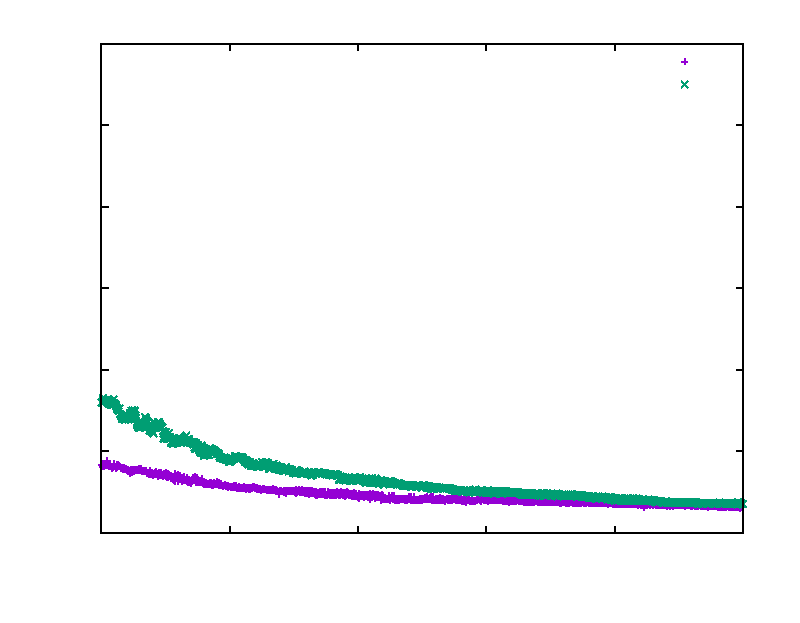
\includegraphics{thesis-performance-size}}%
    \gplfronttext
  \end{picture}%
\endgroup

	\caption{Rendered area size influence on the engine performance in Internet Explorer 11.0}
	\label{performance-size}
\end{figure}

\subsection{Discussion}
Over all was the engine performance rather poor, with the exception of WebKIT based browsers. On the other hand, WebKIT browsers are most common among the users these days\cite{browserstats}. To create a game enjoyable in all currently available browsers, only a limited amount of tiles can be displayed on the screen at all times. Slight improvement may be achieved by further optimization of the engine code, but according to the profiler, most of the execution time is taken up by element bounding box calculation by \texttt{getBBox} function implemented in the browsers\cite{svgtypes}. Other large factor in the engine performance is the browser performing reflow of the layout after most of DOM modifications. In this case might help to rewrite the engine using \emph{React.js}, a recent library that internally creates virtual copy of DOM and then calculates the minimum amount of real DOM changes to save time on reflow\cite{sobo}.

\chapter{Conclusion}
The incentive of this work was curiosity whether the \texttt{svg} element could serve for game graphics rendering in a similar manner to the commonly used \texttt{canvas} element. Both of these elements were introduced as a part of HTML5 standard, but while the latter is used in many modern games, people are discouraged to use for in game environments. The goal was to create an engine allowing to draw isometric graphics for any kind of tile based game. Isometric projection in games is still popular and to sufficient extent allows to display 3D scene using simple 2D rendering. For universal usage the engine needs to strictly separate game logic and assets from the general functionality constant to any game. This entails namely handling the isometric coordinate conversion\footnote{Map model units conversion to screen pixels and back.}, detecting what tiles are currently on the screen and therefore rendering nothing unnecessary. Finally the engine needs to be able to obtain data required to populate the screen with correct tiles and keep those up to date.

Even though the engine implementation attempt was successful and the result meets all requirements, wider application can be hardly recommended. The reason for this discouragement are differences in performance of various web browsers when working with the \texttt{svg} element. As the testing showed, browsers based on WebKIT layout engine, that are currently most widespread among the users, handle SVG in satisfactory speed, but other browsers on the same hardware manage to keep barely playable or even unplayable at all level of frame-rate. Since a developer of a web application can rarely count on the user running certain browser, a game built on the proposed engine would have to carefully limit the amount of displayed tiles and objects. In the view of the fact that no such strict limits are necessary when drawing the graphics to the \texttt{canvas}, it is a better option until the performance equalizes among browser platforms.

\bibliographystyle{csplainnat} % sets plain bibliography style  
\bibliography{sources}     % BibTeX database file  

\appendix
\chapter{Engine implementation source codes}
Source codes of the engine implementation described in Chapter \ref{implementation} is available on GitHub: \href{https://github.com/vit-svoboda/svg-engine}{https://github.com/vit-svoboda/svg-engine}.

\chapter{How to use my engine for your game}
The engine provides API makes the viewport manipulation very easy. The use of this API is demonstrated in the \href{https://github.com/vit-svoboda/svg-engine/tree/master/src/main/webapp/Scripts/game}{sample application}.

\section{Data feed}
Data describing what should be displayed are provided to the engine through an object passed as a first parameter of engine.init method. When engine needs data, methods getData or getDetailedData are called. This data can be obtained from a remote server using HTTP requests, stored in the client memory and passed directly or in any other way suitable for the given game.

\section{Asset management}
To give the game implementation power over what is displayed in place of data discussed earlier, everything displayed is translated using an object passed as a second parameter of the engine.init method. This translation is performed via methods createTile or createObject where the SVG drawing context is provided. Result is placed on the corresponding place in the viewport.

\section{UI handling and game logic}
The third object passed to the engine.init method is responsible for handling user interaction. method createUi is responsible for the standard UI displayed all the time, method processDetailedData is a handler for detailed tile data once it is obtained and method onClick is a handler for any tile or object clicked. Here most of the user interaction needs to be handled. Very little boundaries are given to other interaction implementation though.

\end{document} 